\documentclass[a4paper,11pt,oneside]{book}

%%% το αρχείο αυτό καθορίζει το look που έχουν οι pythonies
%%% γίνεται \input από όλα τα κεφάλαια και τα φύλλα εργασίας

% χρησιμοποιούμενα πακέτα: 
% 
% polyglossia
% xstring
% graphicx
% caption
% xcolor
% hyperref
% minted
% geometry
% titlesec
% datetime
% changepage
% ntheorem

% οριζόμενες εντολές:
%
% smallcaps (βοηθ. removeaccents)
%    μικρά κεφαλαία χωρίς τόνους στα φωνήεντα
% scaling
%    η κλιμάκωση *όλων* των illustrations, τρέχουσα τιμή 0.9
% iconcomputer, iconkeyboard, icondiscuss, iconfillin, iconcaution, iconprompt, dottedline
%    εικονίδια για τα φύλλα εργασίας και εστιγμένη γραμμή
% marginnote
%    πλευρικό σχόλιο
% chapterwabstract (βοηθ. abstract, boxcolor, chaptercolor, concepts, tmpconcepts)
%    εισαγωγικό κείμενο κεφαλαίου με χρωματιστό τετράγωνο, συνοδευτικές έννοιες, κλπ.
% tobecontinued
%    εμφανίζει το "συνεχίζεται στην επόμενη σελίδα"

% οριζόμενα περιβάλλοντα:
% 
% note
%    μια υποσημείωση ή υπόδειξη, με μικρότερα γράμματα
% question
%    μια ερώτηση που "οδηγεί" κάθε νέα ενότητα
% answer
%    μια απάντηση σε μια ερώτηση του φύλλου εργασίας
% theory
%    μια ενότητα "θεωρίας" (στο τέλος ενός κεφαλαίου)
% exercise
%    μια αριθμημένη άσκηση
% step
%    ένα αριθμημένο βήμα (για φύλλο εργασίας)

% για μορφοποίηση κώδικα:
%
% pycode (περιβάλλον)
%     κώδικας python χωρίς αρίθμηση
% pyfile (εντολή)
%     εισαγωγή κώδικα python από αρχείο
% pyfilenl (εντολή)
%     εισαγωγή κώδικα python από αρχείο χωρίς αρίθμηση γραμμών
% pyfilesrc (εντολή)
%    εισαγωγή κώδικα από αρχείο με link στο αρχείο
% pyinline (εντολή)
%     κώδικας python μέσα στη ροή του κειμένου
% pyplain (περιβάλλον, για τα φύλλα εργασίας)
%     κώδικας python χωρίς φόντο
% pynew (περιβάλλον, για τα φύλλα εργασίας)
%     κώδικας python με φόντο
% pyterm (περιβάλλον για τα φύλλα εργασίας)
%     η είσοδος του χρήστη ή τα περιεχόμενα της οθόνης
% pyhighlight (εντολή)
%    highlight κειμένου (χρησιμοποιείται για κώδικα μέσα σε pyplain)


%%% επιλογές γλώσσας και γραμματοσειρών για το XeLaTeX

\usepackage{polyglossia}
\setdefaultlanguage{greek}
\setmainfont[Ligatures=TeX,SmallCapsFont={Linux Libertine O C},SmallCapsFeatures={Letters=SmallCaps}]{Linux Libertine O}
\setsansfont{Linux Biolinum O}
\setmonofont{Ubuntu Mono}
\enablehyphenation

% αφαίρεση τόνων από τα smallcaps
\usepackage{xstring}
\newcommand{\removeaccents}[1]{%
\def\result{#1}%
\StrSubstitute{\result}{ά}{α}[\result]%
\StrSubstitute{\result}{έ}{ε}[\result]%
\StrSubstitute{\result}{ή}{η}[\result]%
\StrSubstitute{\result}{ί}{ι}[\result]%
\StrSubstitute{\result}{ό}{ο}[\result]%
\StrSubstitute{\result}{ύ}{υ}[\result]%
\StrSubstitute{\result}{ώ}{ω}[\result]%
\StrSubstitute{\result}{Ά}{Α}[\result]%
\StrSubstitute{\result}{Έ}{Ε}[\result]%
\StrSubstitute{\result}{Ή}{Η}[\result]%
\StrSubstitute{\result}{Ί}{Ι}[\result]%
\StrSubstitute{\result}{Ό}{Ο}[\result]%
\StrSubstitute{\result}{Ύ}{Υ}[\result]%
\StrSubstitute{\result}{Ώ}{Ω}[\result]%
\result
}

\newcommand{\smallcaps}[1]{\textsc{\removeaccents{#1}}}

%%% εικόνες και λεζάντες

\usepackage{graphicx}
\newcommand{\scaling}{0.9}
\usepackage{caption}
\captionsetup{font=footnotesize}

%%% ειδικά περιβάλλοντα

\usepackage{xcolor}

% ερωτήσεις (που οδηγούν στην επόμενη ενότητα)
\definecolor{questioncolor}{rgb}{0.6,0.5,0.5}
\newenvironment{question}{\noindent\itshape\color{questioncolor}}{\noindent\ignorespaces}

% απαντήσεις (για τις ερωτήσεις των φύλλων εργασίας)
\definecolor{answercolor}{rgb}{0.5,0.5,0.5}
\newenvironment{answer}{\marginnote[16pt]{\iconfillin}\noindent\itshape\color{answercolor}}{\noindent\ignorespaces}

% περιβάλλον "θεωρίας" (πλήρες πλάτος κειμένου)
\usepackage{changepage}
\newenvironment{theory}[1]{\begin{adjustwidth}{}{-\overhang}\smallcaps{#1}\itshape}{\end{adjustwidth}}

% απομεινάρια...
% \newlength{\theoryrulelength}
% \setlength{\theoryrulelength}{36pt}
% \newenvironment{theory}{\rule{\theoryrulelength}{0.4pt}\begin{adjustwidth}{}{-\overhang}\itshape}{\end{adjustwidth}\rule{\theoryrulelength}{0.4pt}}

%%% υπερσύνδεσμοι

\definecolor{linkcolor}{rgb}{0.0,0.5,0.25}
\usepackage[colorlinks=true,urlcolor=linkcolor]{hyperref}

%%% εικονίδια και εστιγμένες γραμμές (για τα φύλλα εργασίας)

\newcommand{\iconcomputer}{
\includegraphics[scale=0.35]{../../share/circle-icons/one-color/computer.eps}}
\newcommand{\iconkeyboard}{
\includegraphics[scale=0.35]{../../share/circle-icons/one-color/keyboard.eps}}
\newcommand{\icondiscuss}{
\includegraphics[scale=0.35]{../../share/circle-icons/one-color/chat.eps}}
\newcommand{\iconfillin}{
\includegraphics[scale=0.35]{../../share/circle-icons/one-color/compose.eps}}
\newcommand{\iconcaution}{
\includegraphics[scale=0.35]{../../share/circle-icons/one-color/caution.eps}}
\newcommand{\iconprompt}{
\includegraphics[scale=0.35]{../../share/circle-icons/one-color/prompt.eps}}
\newcommand{\dottedline}{\vspace{\parskip}\dotfill}

%%% συνεχίζεται στην επόμενη σελίδα

\newcommand{\tobecontinued}{\mbox{}\hfill{\footnotesize ...συνεχίζεται στην επόμενη σελίδα.}}
\newenvironment{note}{\small\upshape}{}

%%% μορφοποίηση κώδικα με το pygmentize

\usepackage{minted}

% fix για ένα bug στο minted που εμφανίζεται όταν χρησιμοποιείται χρώμα στο φόντο (bgcolor)
% http://tex.stackexchange.com/questions/228058/how-to-space-before-and-after-a-minted-code-block-with-bgcolor
\makeatletter
\patchcmd{\minted@colorbg}{\noindent}{\noindent}{}{}
\apptocmd{\endminted@colorbg}{}{}{}
\makeatother

% χρώματα φόντου για τον κώδικα
\definecolor{codebg}{rgb}{0.80,0.95,0.85}
\definecolor{newcodebg}{rgb}{0.75,0.95,0.85}

% ορισμοί για τα περιβάλλοντα κώδικα
% pycode: περιβάλλον κώδικα python χωρίς αρίθμηση
\newminted[pycode]{python3}{bgcolor=codebg}
% pyfile: python από αρχείο
\newmintedfile[pyfile]{python3}{linenos=true,numberblanklines=false,escapeinside=||,bgcolor=codebg}
% pyfilenl: python από αρχείο χωρίς αρίθμηση γραμμών
\newmintedfile[pyfilenl]{python3}{linenos=false,numberblanklines=false,escapeinside=||,bgcolor=codebg}
% pyinline: python μέσα στη ροή του κειμένου
\newmintinline[pyinline]{python3}{linenos=true,numberblanklines=false}
% pyplain: (για τα φύλλα εργασίας) περιβάλλον χωρίς φόντο
\newminted[pyplain]{python3}{bgcolor=white,escapeinside=||,formatcom={\upshape}}
% pynew: (για τα φύλλα εργασίας) περιβάλλον με φόντο
\newminted[pynew]{python3}{bgcolor=newcodebg,escapeinside=||,formatcom={\upshape}}
% pyterm: (για τα φύλλα εργασίας) περιβάλλον για τα περιεχόμενα της οθόνης
\newminted[pyterm]{text}{bgcolor=white,escapeinside=||}

%\newminted[pyterm]{text}{escapeinside=||}
% [TODO] fix: το pyterm χωρίς bgcolor εμφανίζει μεγαλύτερα περιθώρια (πάνω και κάτω) και δεν φαίνεται ωραίο. Το bgcolor είναι προσωρινό workaround, έχει κι αυτό margins (για να μην είναι κολλητά ο κώδικας με το περιθώριο) κι έτσι ο κώδικας στ' αριστερά δεν είναι τέλεια στοιχισμένος.

% εντολή για κώδικα από αρχείο με link στο αρχείο
\newcommand{\pyfilesrc}[2][]{%
\pyfile[#1]{#2}\\
\mbox{}\hfill{\scriptsize\href{http://pythonies.mysch.gr/#2}{\url{#2}}}
}

% εντολή για το highlighting του κώδικα (συνήθως σε pyplain περιβάλλον με escapeinside)
\newcommand{\pyhighlight}[1]{\colorbox{newcodebg}{#1}}

%%% αριθμημένα περιβάλλοντα

\usepackage{ntheorem}

% άσκηση
\makeatletter
\theoremheaderfont{\upshape}%\upshape\bfseries\scshape}
\theorembodyfont{\itshape}%\slshape}
\newtheoremstyle{lmargin}%
  {\item[\theorem@headerfont \llap{##2}\hskip\labelsep\hskip-6pt]}%
  {\item[\theorem@headerfont \llap{##2}\hskip\labelsep ##1\ (##3)\theorem@separator]}
\makeatother
\theoremstyle{lmargin}
\newtheorem{exercise}{}[chapter]

% βήμα φύλλου εργασίας
\makeatletter
\theoremheaderfont{\bfseries}%\upshape\bfseries\scshape}
\theorembodyfont{\upshape}%\slshape}
\newtheoremstyle{lmarginup}%
  {\item[\theorem@headerfont \llap{##2}\hskip\labelsep\hskip-6pt]}%
  {\item[\theorem@headerfont \llap{##2}\hskip\labelsep ##1\ (##3)\theorem@separator]}
\newtheoremstyle{slmarginup}%
  {\item[\theorem@headerfont \llap{##1##2.}\hskip\labelsep\hskip-6pt]}%
  {\item[\theorem@headerfont \llap{##2.}\hskip\labelsep ##1\ (##3)\theorem@separator]}
\makeatother

% deprecated: \newcommand{\standalone}{} to define standalone
%\ifdefined\standalone
    \theoremstyle{slmarginup}
    \newtheorem{step}{}
%\else
%    \theoremstyle{lmarginup}
%    \newtheorem{step}{}[chapter]
%\fi

%%% γεωμετρία σελίδας και συναφείς ορισμοί από το tufte-latex
%%% https://tufte-latex.github.io/tufte-latex/

% εσοχή και διάστημα μεταξύ παραγράφων
% δεν επηρρεάζει το tufte-latex
\parindent=0pt
\parskip=6pt

% γεωμετρία σελίδας και ορισμός μηκών
\usepackage[a4paper,left=24.8mm,top=27.4mm,headsep=2\baselineskip,textwidth=107mm,marginparsep=8.2mm,marginparwidth=49.4mm,textheight=66\baselineskip,headheight=\baselineskip]{geometry}

\setlength{\marginparpush}{12pt}
\addtolength{\marginparpush}{\parskip}
\newlength{\fullwidth}
\setlength{\fullwidth}{\textwidth}
\addtolength{\fullwidth}{\marginparsep}
\addtolength{\fullwidth}{\marginparwidth}
\newlength{\overhang}
\setlength{\overhang}{\marginparsep}
\addtolength{\overhang}{\marginparwidth}

% απομεινάρια...
%\setlength\abovedisplayskip{6pt plus 2pt minus 4pt}
%\setlength\belowdisplayskip{6pt plus 2pt minus 4pt}

% italicize description run-in headings (instead of the default bold)
\renewcommand*\descriptionlabel[1]{\hspace\labelsep\normalfont\em #1}

% πλευρική σημείωση
\newcommand\marginnote[2][0pt]{%
  \marginpar{\hbox{}\vspace*{#1}\vspace*{-1\baselineskip}\noindent \footnotesize\textup{#2}}%
  {}%
}

% formatting title sections
\setcounter{secnumdepth}{-1}

\usepackage{titlesec}
\usepackage[nodate]{datetime}
\newlength{\beforesection}
\setlength{\beforesection}{3ex plus 0.5ex minus 0.2ex}
\addtolength{\beforesection}{-\parskip}
\newlength{\aftersection}
\setlength{\aftersection}{1.5ex plus 0.2ex}
\addtolength{\aftersection}{-\parskip}
\titlespacing*{\section}{0pt}{\beforesection}{\aftersection}

% απομεινάρια...
%\titlespacing*{\chapter}{0pt}{50pt}{40pt}
%\titlespacing*{\section}{0pt}{3.5ex plus 1ex minus .2ex}{2.3ex plus .2ex}

%%% για εισαγωγικό κείμενο κεφαλαίου με χρωματιστό τετράγωνο, συνοδευτικές έννοιες, κλπ.

\newcommand{\abstract}{}
\newcommand{\boxcolor}{}
\newcommand{\chaptercolor}{}
\newcommand{\concepts}{}
\newcommand{\tmpconcepts}{}
\newif\ifbonus

% reference: \titleformat{ command }[ shape ]{ format }{ label }{ sep }{ before-code }[ after-code ]
\titleformat{\chapter}[block]
{\Huge\sffamily}
{}
{0pt}
{\ifbonus\marginnote[-6pt]{\fcolorbox{\boxcolor}{\chaptercolor}{\makebox(40,40){\strut\textcolor{\boxcolor}{\Huge\thechapter}}}\\\vspace{\parskip}\\\tiny\today\\ \currenttime}\else\marginnote[-6pt]{\colorbox{\boxcolor}{\makebox(40,40){\strut\textcolor{\chaptercolor}{\Huge\thechapter}}}\\\vspace{\parskip}\\\tiny\today\\ \currenttime}\fi}
[\small\rmfamily\textmd\abstract\vspace{\parskip}\concepts\vspace{\parskip}\\\mbox{}\hrulefill]

\newcommand{\chapterwabstract}[5]{
	\renewcommand{\abstract}{#2}
    \renewcommand{\tmpconcepts}{#3}
	\ifdefempty{\tmpconcepts}{\renewcommand{\concepts}{}}{\renewcommand{\concepts}{\\\textbf{Έννοιες: }\tmpconcepts}}
	\renewcommand{\boxcolor}{#4}
	\renewcommand{\chaptercolor}{#5}
	\chapter{#1}
}

\definecolor{introColor}{rgb}{0.25,0.5,0.75}
\definecolor{answerColor}{rgb}{0.25,0.75,0.5}
\definecolor{crapsColor}{rgb}{0.5,0.75,0.25}
\definecolor{subtractionColor}{rgb}{0.5,0.25,0.75}
\definecolor{guessColor}{rgb}{0.75,0.25,0.5}
\definecolor{nimColor}{rgb}{0.75,0.5,0.25}
\definecolor{planetColor}{rgb}{0.25,0.25,0.75}
\definecolor{hangmanColor}{rgb}{0.25,0.75,0.25}
\definecolor{oxoColor}{rgb}{0.75,0.25,0.25}

\setcounter{part}{1}
\setcounter{chapter}{1}

%%% DOCUMENT START

\begin{document}

\chapterwabstract{Η Απάντηση}{Στο κεφάλαιο αυτό θα γνωρίσουμε τα βασικά είδη εντολών που θα επιτρέπουν στα προγράμματά μας να \emph{αλληλεπιδρούν} με το χρήστη, δηλαδή να του εμφανίζουν μηνύματα στην οθόνη και να του ζητούν να εισάγει τιμές από το πληκτρολόγιο. Θα κάνουμε επίσης μια πρώτη γνωριμία με ορισμένες θεμελιώδεις έννοιες τις οποίες θα συναντήσουμε συχνά και στα επόμενα κεφάλαια. Κυρίως όμως θα μάθουμε την Απάντηση για τη Ζωή, το Σύμπαν και τα Πάντα!

Πληκτρολογήστε τις εντολές που ακολουθούν. Ίσως να μην είναι άμεσα κατανοητό πώς λειτουργούν, αλλά αυτό είναι φυσιολογικό και η βαθύτερη κατανόηση θα έρθει με την εξάσκηση και τον πειραματισμό. Σκοπός είναι να εξοικειωθείτε με τη γλώσσα, τις λεπτομέρειες της σύνταξής της και τα βασικά της χαρακτηριστικά. Πειραματιστείτε ελεύθερα και μην απογοητεύεστε αν κάνετε λάθη: η προσπάθεια να τα εντοπίσετε και να τα εξαλείψετε είναι κι αυτή κομμάτι του προγραμματισμού.
}{είσοδος, έξοδος, μεταβλητές, δομή επιλογής.}{answerColor}{white}

Ο Douglas Adams, στο βιβλίο The Hitchhiker's Guide to the Galaxy, γράφει για μια υπερευφυή φυλή η οποία, κουρασμένη από τις διαφωνίες σχετικά με το νόημα της ζωής, αποφάσισε να φτιάξει έναν υπολογιστή που θα έδινε οριστικά την απάντηση που αναζητούσαν. Ο υπολογιστής χρειάστηκε 7.5 εκατομμύρια χρόνια για να υπολογίσει και να ελέγξει την Απάντηση \emph{για τη Ζωή, το Σύμπαν και τα Πάντα}. Η Απάντηση ήταν... σαράντα δύο.

Ο υπολογιστής λέγονταν Deep Thought και μπορούμε να φτιάξουμε κι εμείς ένα πρόγραμμα σαν το δικό του. Επειδή δεν διαθέτουμε ανάλογη υπολογιστική ισχύ κι επειδή γνωρίζουμε ήδη την Απάντηση, θα κλέψουμε λίγο: το πρόγραμμά μας δεν θα υπολογίζει την Απάντηση, αλλά μόνο θα την ανακοινώνει στο χρήστη.

%%%%%%%%

\section{Πες Τουλάχιστον Μια Καλημέρα}

Ας ξεκινήσουμε με το πρώτο πράγμα που λέει ο Deep Thought όταν επανέρχεται μετά από 7.5 εκατομμύρια χρόνια: ένα ``Kαλημέρα''.

\marginnote[-64pt]{Ο,τιδήποτε ακολουθεί το σύμβολο \# είναι ένα \emph{σχόλιο}. Δεν αφορά τον υπολογιστή και αγνοείται κατά την εκτέλεση του προγράμματος. Απευθύνεται σε εκείνους που διαβάζουν τον κώδικα και (πρέπει να) χρησιμεύει στην καλύτερη κατανόησή του.}
\marginnote{Για να εμφανίσουμε ένα μήνυμα στην οθόνη χρησιμοποιούμε την \pyinline{print()}, δίνοντας ανάμεσα στις παρενθέσεις το μήνυμα που θα εμφανιστεί.}%
\pyfile[firstline=1,lastline=2]{src/answer.1.py}
\clearpage

Είναι εκπληκτικό ότι σχεδόν σε κάθε βιβλίο για τον προγραμματισμό, αυτό είναι το πρώτο παράδειγμα που συναντάει κανείς: πως να κάνει τον υπολογιστή του να πει μια καλημέρα.

%%%%%%%%

\section{Πες και την Απάντηση}

Στη συνέχεια, ο Deep Thought μπορεί να εμφανίσει την Απάντηση.

\begin{pycode}
# εμφάνιση της Απάντησης
print("Η Απάντηση είναι... 42")
\end{pycode}

Το ίδιο αποτέλεσμα μπορεί να επιτευχθεί και με διαφορετικό τρόπο.

\marginnote[18pt]{Μπορούμε να εμφανίσουμε με την \pyinline{print()} πολλές τιμές, αρκεί να τις χωρίσουμε με κόμμα. Ανάμεσά στις τιμές εμφανίζεται ένα κενό, όμως αυτή η προκαθορισμένη συμπεριφορά είναι δυνατόν ν' αλλάξει.}
\pyfilesrc[firstline=3,lastline=5]{src/answer.1.py}

Ενώ ο χρήστης βλέπει το ίδιο μήνυμα στην οθόνη, οι δύο \pyinline{print()} δεν κάνουν το ίδιο πράγμα. Η πρώτη εμφανίζει \emph{πάντα} την τιμή 42, ενώ η δεύτερη εμφανίζει την τιμή \pyinline{answer}, \emph{όποια κι αν είναι αυτή}.

\marginnote[18pt]{\begin{center}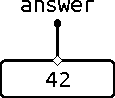
\includegraphics[scale=\scaling]{illustrations/variable.pdf}\end{center}
Η μεταβλητή \pyinline{answer} έχει την τιμή \pyinline{42}. Εναλλακτικά, θα λέγαμε ότι στην τιμή \pyinline{42} έχει δοθεί το όνομα \pyinline{answer}.}
Η \pyinline{answer} είναι μια \emph{μεταβλητή}. Μπορούμε να πούμε ότι δίνουμε στην τιμή 42 το όνομα \pyinline{answer}. Μπορούμε επίσης να πούμε ότι δίνουμε στο όνομα \pyinline{answer} την τιμή 42. Και οι δύο περιγραφές είναι ορθές, είναι απλά θέμα οπτικής γωνίας. 
Σημασία έχει ότι οι μεταβλητές επιτρέπουν στα προγράμματά μας να διατηρούν, να \emph{``θυμούνται''} τις τιμές που είναι σημαντικές. Όταν συσχετίζουμε μια τιμή μ' ένα όνομα (όπως κάνουμε εδώ με το όνομα \pyinline{answer} και την τιμή 42) μπορούμε ν' αναφερθούμε σε αυτή κι αργότερα, διαφορετικά δεν έχουμε τρόπο ανάκτησής της.

%Η εντολή \pyinline{answer = 42} δεν είναι δήλωση, δεν διατυπώνει κάτι που πρέπει να ισχύει για πάντα. Με μια αντίστοιχη εντολή μπορούμε στη συνέχεια να αλλάξουμε την τιμή της μεταβλητής \pyinline{answer}, να δώσουμε αυτό το όνομα σε άλλη τιμή (αν και αυτό δε θα χρειαστεί στο πρόγραμμά μας, γιατί η Απάντηση είναι μία).

%%%%%%%%

\section{Για Περίμενε Λιγάκι}

\begin{question}
Πώς γίνεται να προσθέσουμε λίγο σασπένς; Μπορούμε να εισάγουμε μια καθυστέρηση λίγο πριν την ανακοίνωση της Απάντησης;
\end{question}

Επειδή στις βασικές εντολές της Python δεν συγκαταλέγεται κάποια εντολή καθυστέρησης, θα χρησιμοποιήσουμε μια \emph{βιβλιοθήκη}, η οποία παρέχει τη λειτουργικότητα που μας χρειάζεται. Οι βιβλιοθήκες περιέχουν έτοιμο κώδικα και τις συναντάμε στις περισσότερες γλώσσες προγραμματισμού: είναι συλλογές από μικρά προγράμματα που μπορούμε να χρησιμοποιήσουμε στα προγράμματά μας.

%Καθορίζοντας την τιμή της αντίστοιχης παραμέτρου \pyinline{sep}, μπορούμε να αλλάξουμε το προκαθορισμένο κενό που εμφανίζεται ανάμεσα στις παραμέτρους της \pyinline{print()}.
\marginnote[18pt]{Για να χρησιμοποιήσουμε μια βιβλιοθήκη θα πρέπει πρώτα να την εισάγουμε (\pyinline{import}). Εδώ θα εισάγουμε τη βιβλιοθήκη \pyinline{time} (που περιέχει έτοιμα υποπρογράμματα για τη διαχείριση του χρόνου) και θα χρησιμοποιήσουμε την \pyinline{sleep()}, που καθυστερεί την εκτέλεση του προγράμματος για όσα δευτερόλεπτα καθορίσουμε.}
\pyfilesrc{src/answer.2.py}
\clearpage

Αν θέλουμε να υπάρχει πραγματικό σασπένς και να είμαστε πιστοί στο βιβλίο του Douglas Adams, θα πρέπει να εισάγουμε μια καθυστέρηση της τάξης των 7.5 εκατομυρίων ετών (σε δευτερόλεπτα). Ίσως δεν θα έπρεπε να δοκιμάσετε τον κώδικα που ακολουθεί, μπορεί να βαρεθείτε λιγάκι μέχρι να εμφανιστεί η Απάντηση.

\marginnote[18pt]{Το σύμβολο \pyinline{*} αντιστοιχεί στην πράξη του πολλαπλασιασμού. Σε άλλες εκφράσεις μπορείτε επίσης να χρησιμοποιήσετε τα κλασικά \pyinline{+} και \pyinline{-}, καθώς επίσης και το \pyinline{/} για τη διαίρεση, το \pyinline{//} για το πηλίκο της ακέραιας διαίρεσης και το \% για το υπόλοιπο της ακέραιας διαίρεσης.}
\marginnote{Αν θέλετε να διακόψετε την εκτέλεση ενός προγράμματος, χρησιμοποιήστε τον συνδυασμό πλήκτρων Ctrl+C.}
\marginnote{\begin{center}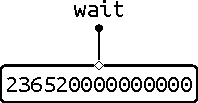
\includegraphics[scale=\scaling]{illustrations/computed.pdf}\end{center}}
\pyfilesrc[firstline=4,lastline=9]{src/answer.3.py}

Στον παραπάνω κώδικα η τιμή της μεταβλητής \pyinline{wait} αντιστοιχεί στα δευτερόλεπτα καθυστέρησης και, σε αντίθεση με την \pyinline{answer}, δεν καθορίζεται απευθείας αλλά προκύπτει από τον \emph{υπολογισμό} της τιμής ενός γινομένου. 
%Η εντολή \pyinline{wait = 7500000 * 365 * 24 * 60 * 60} σημαίνει: υπολόγισε την τιμή της παράστασης \pyinline{7500000 * 365 * 24 * 60 * 60} κι ονόμασε το αποτέλεσμα \pyinline{wait}.

%%%%%%%%

\section{Πιάσαμε την Κουβέντα}

\begin{question}
Μέχρι στιγμής ο Deep Thought είναι λίγο απρόσωπος: απλά ανακοινώνει την Απάντηση. Ο χρήστης δεν θα αλληλεπιδρά με το πρόγραμμα;
\end{question}

Η ροή της πληροφορίας ανάμεσα στο πρόγραμμα και τον χρήστη είναι μονόδρομη. Στις περισσότερες περιπτώσεις ένα πρόγραμμα δεν περιορίζεται στην εμφάνιση μηνυμάτων, αλλά χρειάζεται και να κάνει ερωτήσεις στον χρήστη, να του ζητήσει τιμές.

Θα προγραμματίσουμε τον Deep Thought έτσι ώστε να ζητάει το όνομα του χρήστη και να τον καλημερίζει κατάλληλα. Έτσι θα έχουν ένα στοιχειώδη διάλογο, πριν από την ανακοίνωση της Απάντησης.

\marginnote[18pt]{Για να εμφανίσουμε ένα κενό στο τέλος του μηνύματος, αντί για την προκαθορισμένη αλλαγή γραμμής, ορίζουμε την παράμετρο \pyinline{end} της \pyinline{print()} να είναι ίση με το κενό.}
\marginnote{Για να ζητήσουμε μια τιμή από το πληκτρολόγιο χρησιμοποιούμε την \pyinline{input()}, η οποία επιστρέφει μια \emph{αλφαριθμητική} τιμή: το κείμενο που πληκτρολογήθηκε από τον χρήστη.}
%\marginnote{Κάθε τιμή έχει συγκεκριμένο \emph{τύπο}. Οι ακέραιες τιμές είναι τύπου \pyinline{int}, ενώ οι αλφαριθμητικές είναι τύπου \pyinline{str}. Κάθε αλφαριθμητική τιμή περικλείεται σε εισαγωγικά (μονά ή διπλά). Τα μηνύματα που εμφανίσαμε μέχρι τώρα περικλείονται σε εισαγωγικά επειδή είναι αλφαριθμητικές τιμές.}

\pyfilesrc[firstline=2,lastline=6]{src/answer.4.py}

Εναλλακτικά:

\marginnote{Η εμφάνιση ενός μηνύματος πριν την ανάγνωση τιμών είναι τόσο συνηθισμένη που η \pyinline{input()} μπορεί να δεχθεί ανάμεσα στις παρενθέσεις το μήνυμα που πρέπει να εμφανιστεί.}%
\begin{pycode}
# είσοδος ονόματος
name = input("Πώς σε λένε; ")
# χαιρετισμός
print("Καλημέρα", name)
\end{pycode}

Η τιμή της μεταβλητής \pyinline{name} είναι το κείμενο που πληκτρολογεί ο χρήστης και φυσικά δεν είναι γνωστό εκ των προτέρων. O Deep Thought χρησιμοποιεί την τιμή της μεταβλητής \pyinline{name} για να καλημερίσει τον χρήστη, \emph{όποια κι αν είναι αυτή η τιμή}.

%Αυτή η μικρή προσθήκη που κάναμε είχε ένα σημαντικό αποτέλεσμα που ίσως να μη γίνεται άμεσα αντιληπτό: το πρόγραμμά μας δεν εμφανίζει πλέον πάντα τα ίδια μηνύματα, αλλά \emph{διαφοροποιεί την έξοδό του με βάση τις τιμές που δέχεται από το χρήστη}.

%%%%%%%%

\section{Έχεις Ώρα;}

\begin{question}
Αν ένας χρήστης εκτελέσει το βράδι το πρόγραμμα που έχουμε φτιάξει για τον Deep Thought, τότε θα δυσκολευτεί να πιστέψει ότι πρόκειται για έναν υπερυπολογιστή που γνωρίζει την Απάντηση για τη Ζωή, το Σύμπαν και τα Πάντα, αφού θα τον χαιρετίσει βραδιάτικα με ένα ``Καλημέρα''. 
\end{question}

Tο πρόγραμμα πρέπει να γνωρίζει την ώρα της ημέρας. Ευτυχώς ο υπολογιστής μας ξέρει τι ώρα είναι, οπότε απλά θα τον ρωτήσουμε.

\marginnote[18pt]{Η \pyinline{localtime()} της βιβλιοθήκης \pyinline{time} επιστρέφει πληροφορίες για την ημερομηνία και την ώρα του συστήματος. Οι συντακτικές λεπτομέρειες δεν έχουν σημασία αυτή την στιγμή.}
\pyfile[firstline=5,lastline=6]{src/answer.5.py}

Εδώ όμως το ουσιαστικό πρόβλημα είναι ότι οι εντολές που θα πρέπει να εκτελέσει το πρόγραμμά μας δεν είναι πάντα οι ίδιες.  Θα πρέπει να προγραμματίσουμε τον Deep Thought έτσι ώστε να \emph{ελέγχει} την ώρα της ημέρας και να εμφανίζει διαφορετικό μήνυμα \emph{ανάλογα με το αποτέλεσμα του ελέγχου}. 

\marginnote[18pt]{Η \pyinline{if} συνοδεύεται από μια \emph{συνθήκη}, η οποία ελέγχεται κατά την εκτέλεση του προγράμματος και μπορεί να είναι αληθής (\pyinline{True}) ή ψευδής (\pyinline{False}).}
\marginnote{Οι εντολές που ακολουθούν την \pyinline{if} είναι στοιχισμένες δεξιότερα από αυτή. Η στοίχιση επιτυγχάνεται εισάγοντας κενά πριν από τις εντολές, τα οποία υποδηλώνουν ότι αυτές οι εντολές θα εκτελεστούν μόνο αν η συνθήκη είναι αληθής. Παρομοίως, οι εντολές που ακολουθούν την \pyinline{else} είναι στοιχισμένες δεξιότερα και θα εκτελεστούν μόνο εφόσον η συνθήκη είναι ψευδής.}
%\marginnote{Το σύμβολο \pyinline{<} χρησιμοποιείται για να συγκρίνει τιμές, όπως και τα \pyinline{<=}, \pyinline{>}, \pyinline{>=}, \pyinline{==} και \pyinline{!=}. Με τα δύο τελευταία ελέγχουμε αν δύο τιμές είναι ίσες ή διαφορετικές.}
\marginnote{Μην παραλείπετε το σύμβολο \pyinline{:} μετά την συνθήκη της \pyinline{if} και την \pyinline{else}.}
\pyfilesrc[firstline=7,lastline=11]{src/answer.5.py}

Ο κώδικας ελέγχει την συνθήκη \pyinline{hour < 14}, δηλαδή αν η τρέχουσα ώρα είναι πριν τις 2 το μεσημέρι. Αν η συνθήκη ισχύει τότε εμφανίζει το μήνυμα \pyinline{"Καλημέρα"}, αλλιώς το μήνυμα \pyinline{"Καλησπέρα"}. Με άλλα λόγια, το πρόγραμμα \emph{επιλέγει} την συμπεριφορά του ανάλογα με τις \emph{συνθήκες} που επικρατούν την ώρα της εκτέλεσής του. Αυτό το νέο προγραμματιστικό εργαλείο ονομάζεται \emph{δομή επιλογής}.

Μια πρακτική συμβουλή: θα πρέπει πάντα να εκτελούμε τα προγράμματά μας, ελέγχοντας ότι η συμπεριφορά τους είναι ορθή. Εδώ το πρόγραμμά μας περιέχει μια δομή επιλογής με δύο πιθανές περιπτώσεις και θα πρέπει να ελέγξουμε ότι λειτουργεί σωστά και στις δύο. Αν το εκτελέσουμε πρωί και μας χαιρετίσει μ' ένα \pyinline{"Καλημέρα"}, δεν είναι καλή ιδέα να περιμένουμε μέχρι το βράδι για να ελέγξουμε αν αλλάζει η συμπεριφορά του.

Η λύση είναι να τροποποιήσουμε \emph{προσωρινά} το πρόγραμμά μας και να καθορίσουμε εμείς την ώρα, αντί να χρησιμοποιήσουμε την ώρα του συστήματος.
Καθορίζοντας ότι είναι 10 το πρωί, το πρόγραμμα θα εμφανίσει το πρώτο μήνυμα. 

\begin{pycode}
# ΓΙΑ ΕΛΕΓΧΟ: ορισμός ώρας
hour = 10
\end{pycode}

Όταν αλλάξουμε την τιμή της μεταβλητής \pyinline{hour} σε 20 τότε, εκτός συγκλονιστικού απροόπτου, θα δούμε το δεύτερο μήνυμα. 

\begin{pycode}
# ΓΙΑ ΕΛΕΓΧΟ: ορισμός ώρας
hour = 20
\end{pycode}

% Αν όλα πάνε καλά με τους ελέγχους μας, επαναφέρουμε το πρόγραμμα στην αρχική του κατάσταση.

% μια if αρκεί για δύο περιπτώσεις. Αργότερα θα πούμε τι γίνεται όταν υπάρχουν περισσότερες.

%%%%%%%%

\section{Πλήρες Τελικό Πρόγραμμα}

\pyfilesrc{src/answer.final.py}

%%%%%%%%

\section*{Και Τώρα Τι;}

Δεν μάθατε και λίγα για αρχή. Ίσως μάλιστα να αισθάνεστε λίγο όπως ο Παπαγάλος, του Ζαχαρία Παπαντωνίου.
\begin{quote}
Σαν έμαθε τη λέξη \emph{καλησπέρα}\\
ο παπαγάλος, είπε ξαφνικά:\\
«Είμαι σοφός, γνωρίζω ελληνικά.\\
Τι κάθομαι εδώ πέρα;»
\end{quote}
Όπου \emph{ελληνικά}, αντικαταστήστε με Pythonιά. Όμως είναι ανάγκη να εμπεδώσετε τις έννοιες που συναντήσατε χρησιμοποιώντας τις σε νέα προβλήματα (δηλαδή λύνοντας τις ασκήσεις που ακολουθούν). Διαφορετικά, θα αισθανθείτε σίγουρα όπως ο Παπαγάλος:
\begin{quote}
«Κυρ παπαγάλε, θα ’χομε την τύχη\\
ν’ ακούσωμε τις λες και πάρα πέρα;»\\
Ο παπαγάλος βήχει, ξεροβήχει...\\
μα τι να πει; Ξανάπε: «καλησπέρα».
\end{quote}

\section{Τροποποιήσεις -- Επεκτάσεις}

Στο πρόγραμμα που κατασκευάσαμε χρησιμοποιήσαμε την \pyinline{input()} για να ζητήσουμε το όνομα του χρήστη. Η τιμή που επιστρέφει η \pyinline{input()} είναι αλφαριθμητική, έχει δηλαδή την μορφή κειμένου. Αυτό δεν είναι πρόβλημα όταν ζητάμε το όνομα του χρήστη γιατί κι αυτό έχει την μορφή κειμένου. Όταν όμως θέλουμε να ζητήσουμε από το χρήστη έναν ακέραιο ή έναν πραγματικό αριθμό (κάτι που θα χρειαστεί στις ασκήσεις που ακολουθούν), τότε θα πρέπει να μετατρέψουμε την αλφαριθμητική τιμή που επιστρέφει η \pyinline{input()} σε αριθμητική, με τον τρόπο που φαίνεται παρακάτω:

\begin{pycode}
# το κείμενο που πληκτρολογεί ο χρήστης
# μετατρέπεται σε ακέραιο αριθμό και 
# αποθηκεύεται στην μεταβλητή number
number = int(input())
\end{pycode}

\begin{pycode}
# το κείμενο που πληκτρολογεί ο χρήστης
# μετατρέπεται σε πραγματικό αριθμό και 
# αποθηκεύεται στην μεταβλητή number
number = float(input())
\end{pycode}

Οι \pyinline{int()} και \pyinline{float()} χρησιμοποιούνται γενικότερα όταν χρειάζεται να μετατρέψουμε μια τιμή σε ακέραια ή πραγματική. Για παράδειγμα, η εκφραση \pyinline{int(3.14159)} έχει την ακέραια τιμή \pyinline{3}.

Κάτι άλλο που θα φανεί χρήσιμο σε κάποιες από τις ασκήσεις είναι ο υπολογισμός του πηλίκου και του υπολοίπου της \emph{ακέραιας} διαίρεσης δύο αριθμών. Αυτό γίνεται όπως στο παράδειγμα:

\begin{pycode}
# πηλίκο ακέραιας διαίρεσης του number με το 10
q = number // 10
# υπόλοιπο ακέραιας διαίρεσης του number με το 2
r = number % 2
\end{pycode}

\begin{exercise}
Μπορείτε να επεκτείνετε το πρόγραμμα του Deep Thought έτσι ώστε να ρωτά το χρήστη ποιο είναι το έτος γέννησής του και να υπολογίζει την ηλικία του. Για να το καταφέρετε αυτό, θα πρέπει το πρόγραμμά σας να γνωρίζει ποιο είναι το τρέχον έτος:

{\upshape 
\begin{pycode}
year = time.localtime().tm_year
\end{pycode}
}

Στη συνέχεια, μπορείτε απλά να εμφανίσετε στο χρήστη την ηλικία του (αν και πιθανότατα θα τη γνωρίζει) ή να χρησιμοποιήσετε την \pyinline{if} για να εμφανίζετε διαφορετικό μήνυμα ανάλογα με την ηλικία.
\end{exercise}

\section{Ασκήσεις}

\begin{exercise}
Στη Σελήνη το βάρος ενός αντικειμένου είναι το $\frac{1}{6}$ του βάρους του στη Γη.
Στην Αφροδίτη το βάρος ενός αντικειμένου είναι 0,9 φορές το βάρος του στη Γη. 
Στον Ήλιο το βάρος ενός αντικειμένου είναι 27,07 φορές το βάρος του στη Γη, αλλά όταν βρίσκεται κανείς εκεί η αύξηση του βάρους δεν είναι το βασικότερο πρόβλημα.
Να γράψετε πρόγραμμα που θα ζητάει από το χρήστη το βάρος του στη Γη και θα εμφανίζει το βάρος του στη Σελήνη, την Αφροδίτη και τον Ήλιο. 
\end{exercise}

\begin{exercise} % Nicomachus
Υπάρχουν πολλά παιχνίδια στα οποία κάποιος σας ζητά να σκεφτείτε έναν μυστικό αριθμό και, μετά από μερικές ερωτήσεις και υπολογισμούς, «μαντεύει» τον αριθμό που είχατε σκεφτεί. Ένα πολύ παλιό παράδειγμα βασίζεται σ' ένα θεώρημα του κινέζου Sun Tzu, που έζησε κάπου ανάμεσα στον 3\textsuperscript{ο} και τον 5\textsuperscript{ο} αιώνα. Ας υποθέσουμε ότι ο άγνωστος αριθμός είναι ο x. Αν ονομάσουμε α, β και γ τα υπόλοιπα της διαίρεσης του x με το 3, το 5 και το 7 αντίστοιχα, τότε για να βρούμε τον άγνωστο αριθμό θα πρέπει να υπολογίσουμε την τιμή της παράστασης 70α + 21β + 15γ και στη συνέχεια να διαιρέσουμε με το 105. Το υπόλοιπο της διαίρεσης θα είναι ο μυστικός αριθμός. Να αναπτύξετε ένα πρόγραμμα το οποίο ζητάει από το χρήστη να σκεφτεί έναν μυστικό αριθμό από το 1 μέχρι και το 100. Στη συνέχεια, το πρόγραμμα ρωτάει το χρήστη ποιο είναι το υπόλοιπο της διαίρεσης αυτού του αριθμού με το 3, το 5 και το 7 και ανακοινώνει τον μυστικό αριθμό, αφήνοντας το χρήστη έκπληκτο με τις υπερφυσικές του ικανότητες.
\end{exercise}

\begin{exercise}
\marginnote[18pt]{
}Να γράψετε πρόγραμμα που θα ζητάει από το χρήστη το πλήθος των δευτερολέπτων που έχουν περάσει από τα μεσάνυχτα και θα εμφανίζει την τρέχουσα ώρα στη μορφή \emph{ώρες:λεπτά:δευτερόλεπτα}. Για παράδειγμα, αν ο χρήστης καθορίσει ότι έχουν περάσει 42222 δευτερόλεπτα από τα μεσάνυχτα, το πρόγραμμα θα απαντά ότι η ώρα είναι 11:43:42.

\begin{note}
Σημείωση: Αν οι ώρες, τα λεπτά ή τα δευτερόλεπτα είναι μονοψήφιοι αριθμοί τότε η ώρα δεν θα εμφανίζεται «όμορφα». Αν αυτό προσβάλλει την αισθητική σας και δεν μπορείτε να το ανεχτείτε, έχετε υπόψη ότι μπορείτε να εμφανίσετε έναν αριθμό ως διψήφιο, με ένα αρχικό μηδέν όταν είναι απαραίτητο, με τον εξής φρικτό τρόπο:

\begin{pycode}
# έστω num ένας ακέραιος, πιθανώς μονοψήφιος
# έτσι εμφανίζεται με αρχικό μηδέν, αν χρειάζεται
print("{:02}".format(num))
\end{pycode}
\end{note}

% (datetime.datetime.now() - datetime.datetime.combine(datetime.date.today(),datetime.time(0,0,0))).total_seconds()
%
% now = datetime.datetime.now()
% midnight = datetime.datetime.combine(now.date(),datetime.time(0))
% s = (now - midnight).total_seconds() 
\end{exercise}

%%%%%%%%

\section*{}
\vspace{2\parskip}
\hrulefill

\begin{theory}{Έξοδος}
Η εμφάνιση μηνυμάτων και γενικότερα η ροή πληροφορίας από ένα πρόγραμμα προς το περιβάλλον του ονομάζεται \emph{έξοδος}.
% Στην Python για την έξοδο χρησιμοποιείται η συνάρτηση \pyinline{print()}.

\end{theory}

\begin{theory}{Είσοδος}
Η ανάγνωση των τιμών που πληκτρολογεί ο χρήστης και γενικότερα η ροή πληροφορίας προς ένα πρόγραμμα από το περιβάλλον του ονομάζεται \emph{είσοδος}.
%Στην Python για την είσοδο χρησιμοποιείται η συνάρτηση \pyinline{input()}.
\end{theory}

\begin{theory}{Μεταβλητές}
%\marginnote{Εδώ θα βάλουμε ένα ωραίο σχήμα.}
Μεταβλητή είναι το όνομα που δίνει ο προγραμματιστής σε μια τιμή ή ένα αντικείμενο. Χρειαζόμαστε τις μεταβλητές για τον ίδιο λόγο που χρειαζόμαστε γενικά τα ονόματα: για να μπορούμε να αναφερθούμε σε αυτές τις τιμές, ακόμα και όταν δεν γνωρίζουμε ή δεν έχει σημασία ποιες ακριβώς είναι αυτές.
% ακόμα και για να μπορούμε να τις αλλάξουμε.
%Στο παράδειγμά μας, το όνομα είναι \pyinline{answer} και η τιμή είναι \pyinline{42}. Δίνουμε όνομα στην Απάντηση για να μπορούμε να αναφερθούμε σε αυτήν, όποια και αν είναι η τιμή της. 
Η τιμή στην οποία αναφέρεται ένα όνομα, η τιμή της μεταβλητής, μπορεί να αλλάξει καθώς εκτελείται ένα πρόγραμμα. Είναι καλή πρακτική να επιλέγουμε περιγραφικά ονόματα για τις μεταβλητές μας, ονόματα που υποδηλώνουν το είδος των τιμών στις οποίες αντιστοιχούν. 
%%% Συχνά θεωρούμε ότι στις μεταβλητές αποθηκεύονται τιμές.
\end{theory}

\begin{theory}{Δομή Επιλογής}
Η δομή επιλογής δίνει τη δυνατότητα στα προγράμματά μας να ελέγχουν \emph{συνθήκες} και να διαφοροποιούν την συμπεριφορά τους ανάλογα με αυτές. Χωρίς αυτή τη δυνατότητα, τα προγράμματά μας εκτελούν πάντα τις ίδιες εντολές, με την ίδια σειρά και αυτό τους στερεί την προσαρμοστικότητα ή την ``εξυπνάδα'' που είναι απαραίτητη ακόμα και σε πολύ απλά προβλήματα.
\end{theory}

\begin{theory}{Σκουπίδια Μπαίνουν, Σκουπίδια Βγαίνουν}
Στο βιβλίο, ο Deep Thought προσφέρει μια εξήγηση για το παράδοξο της Απάντησης: ``Για να είμαι ειλικρινής, πιστεύω ότι το πρόβλημα είναι ότι ποτέ δεν γνωρίζατε πραγματικά ποια είναι η ερώτηση. Αν μάθετε την ερώτηση, τότε θα καταλάβετε τι σημαίνει και η απάντηση.'' Τα προγράμματα τα γράφουν προγραμματιστές. Άνθρωποι. Οι υπολογιστές απλά τα εκτελούν κι ελπίζουμε ότι η απάντηση που μας δίνουν αποτελεί τη λύση στο πρόβλημά μας. Για να γίνει όμως αυτό, θα πρέπει οι προγραμματιστές να έχουν κατανοήσει σωστά το πρόβλημα, οι οδηγίες που έχουν καθορίσει να είναι ορθές και τα δεδομένα που παρέχουν οι χρήστες να έχουν νόημα. Σε διαφορετική περίπτωση, η απάντηση θα μας είναι άχρηστη. Ο Charles Babbage, ο άνθρωπος που σχεδίασε έναν μηχανικό προγραμματιζόμενο υπολογιστή εκατό χρόνια πριν κατασκευαστούν οι πρώτοι ηλεκτρονικοί υπολογιστές, είχε γράψει: ``Σε δύο περιπτώσεις έχω ερωτηθεί: Πείτε μας κύριε Babbage, αν εισάγετε λάθος νούμερα στη μηχανή, θα βγουν οι σωστές απαντήσεις; ... Δεν μπορώ να συλλάβω τι είδους σύγχυση ιδεών θα προκαλούσε μια τέτοια ερώτηση.''
\end{theory}

\hrulefill

\end{document}
